% GENI Lab_2.tex - GENI Lab 1 for Cloud Computing class (Spring 2015)
% Chanmann Lim - March 2015

\documentclass[a4paper]{article}

\usepackage[margin=1 in]{geometry}
\usepackage{listings}
\usepackage{graphicx}
\usepackage{float}

\begin{document}
\title{CS 7001-03: Report for GENI Lab 2 - Instrumentation and Measurement of a GENI Slice}
\author{Chanmann Lim\\ 
	\texttt{cl9p8@mail.mail.missouri.edu}}
\date{March 10, 2015}
\maketitle

% ---------------------------------------- 1 ----------------------------------------
\paragraph{1. } Screenshots of OnTimeMeasure instance's Graphite page:
\begin{figure}[H]
  \centering
    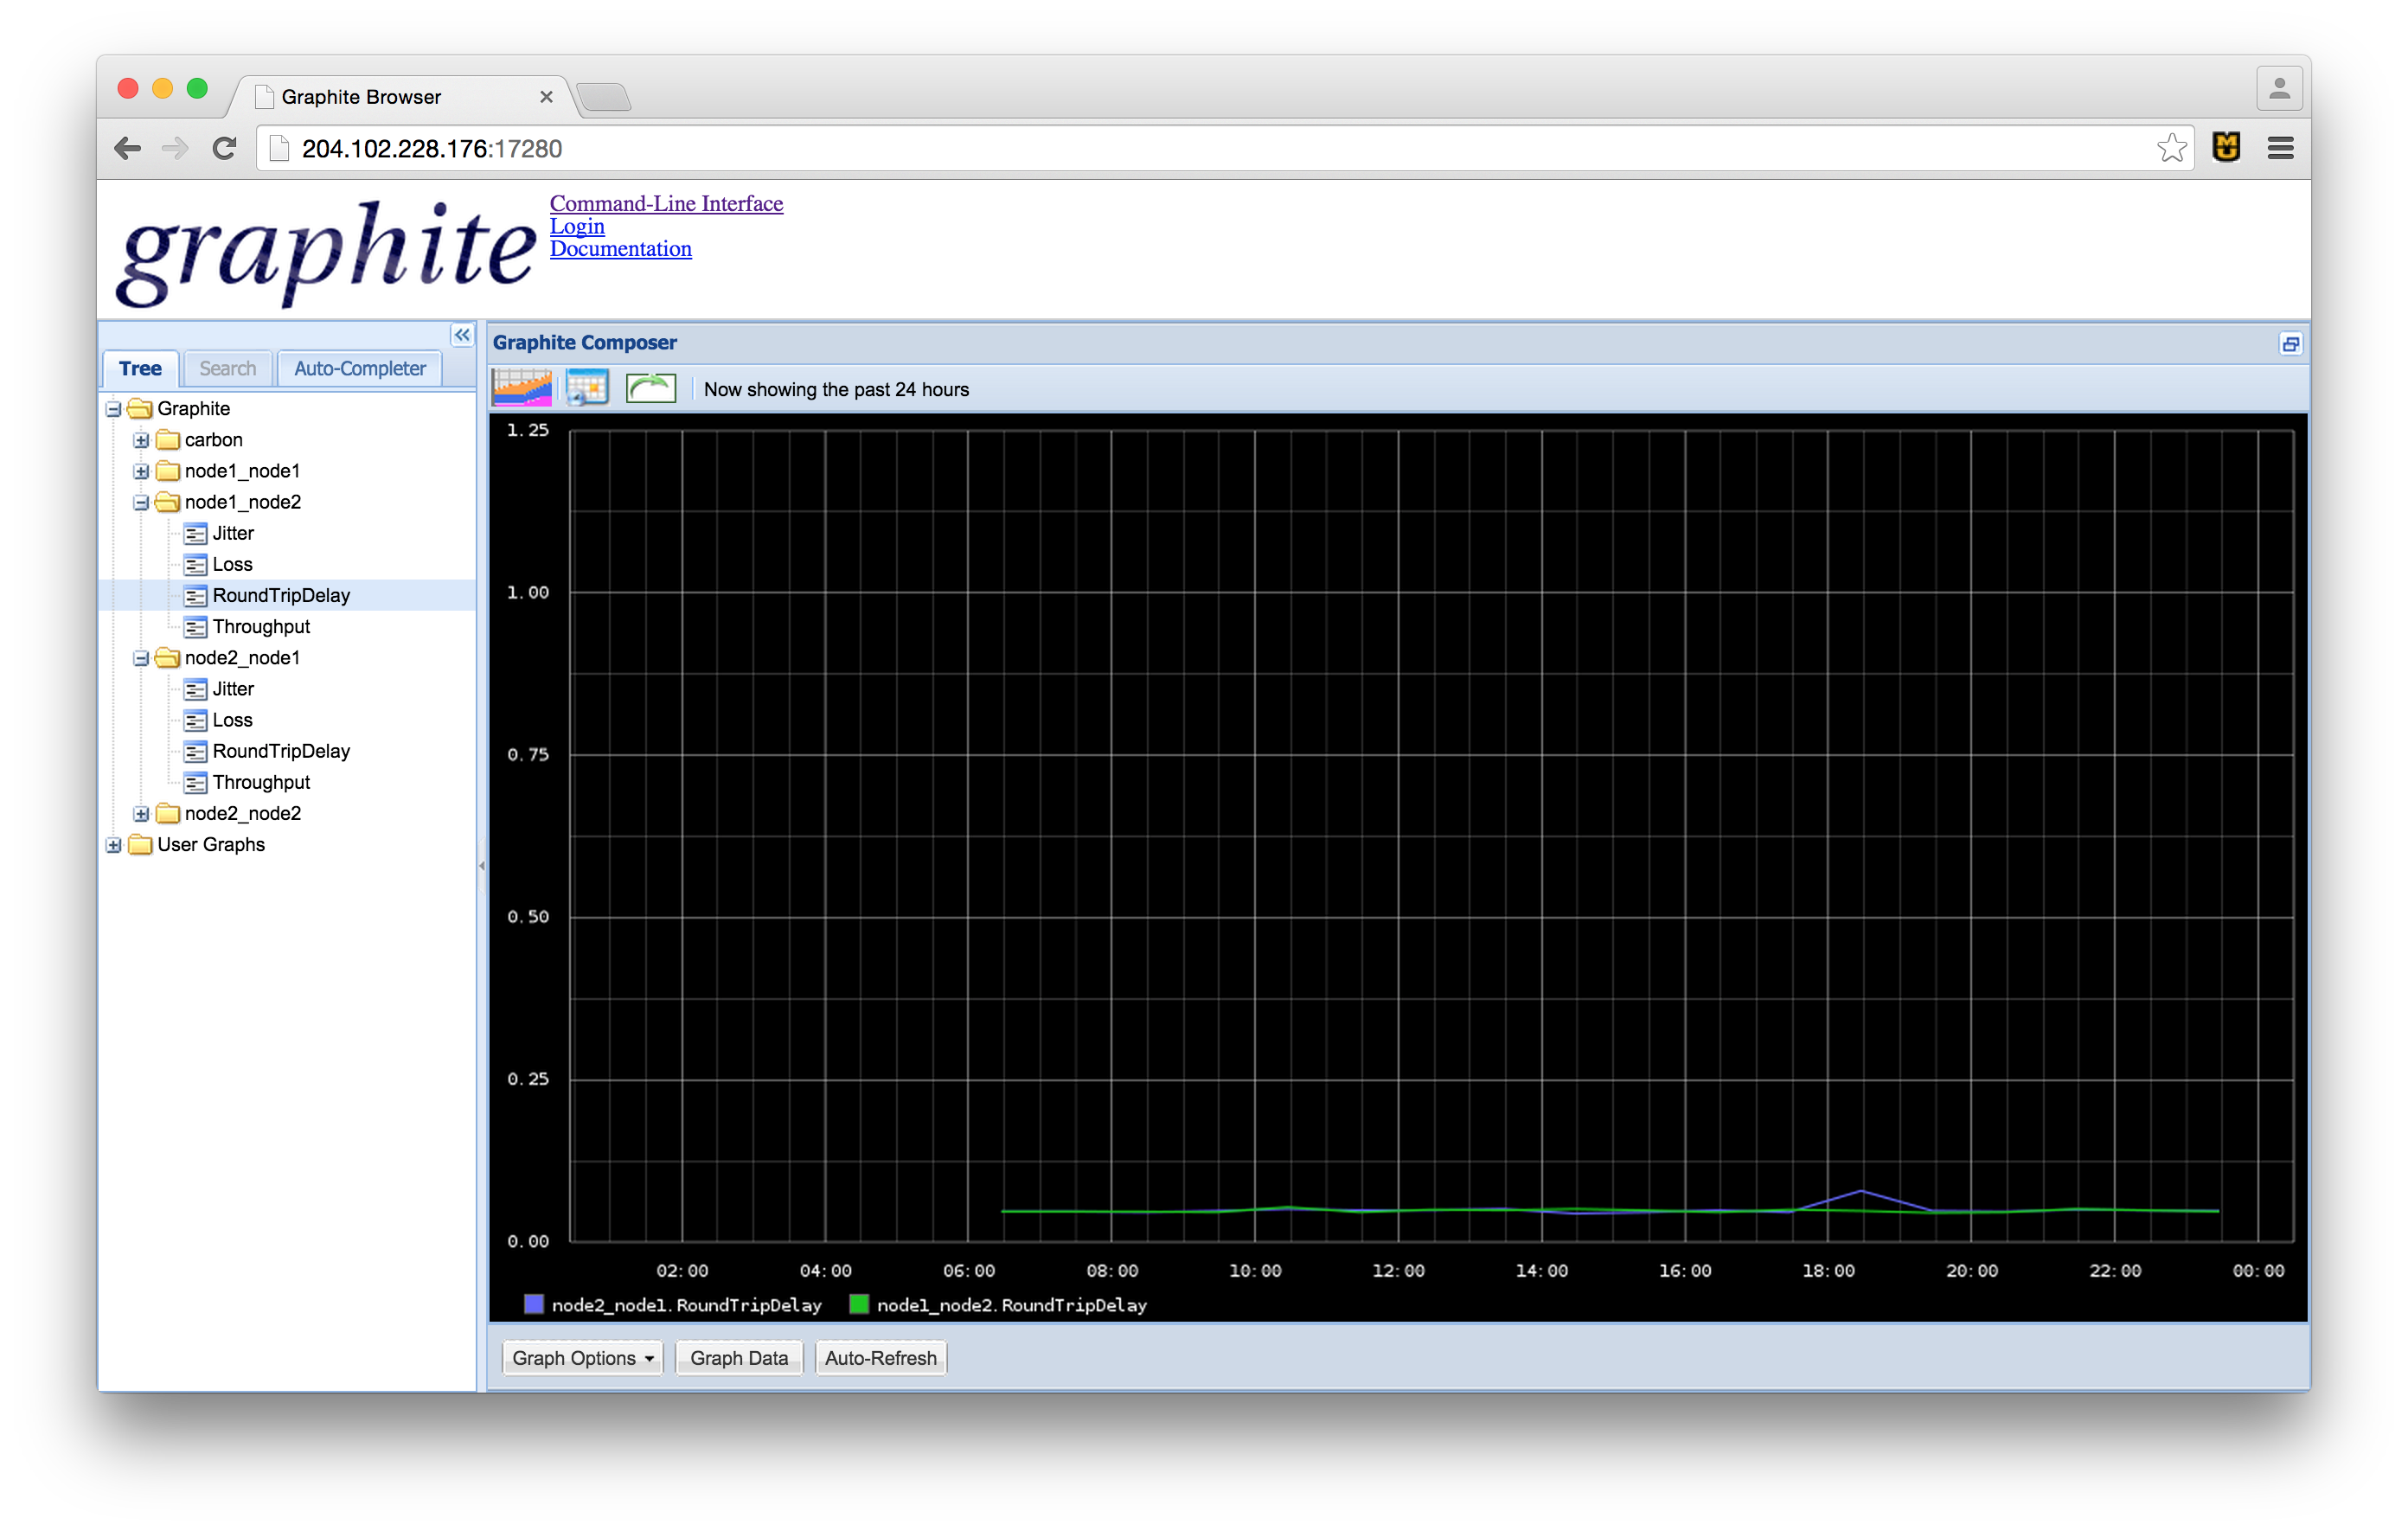
\includegraphics[scale=.32]{round_trip_delay.png}
  \caption{RoundTripDelay}
\end{figure}
\begin{figure}[H]
  \centering
    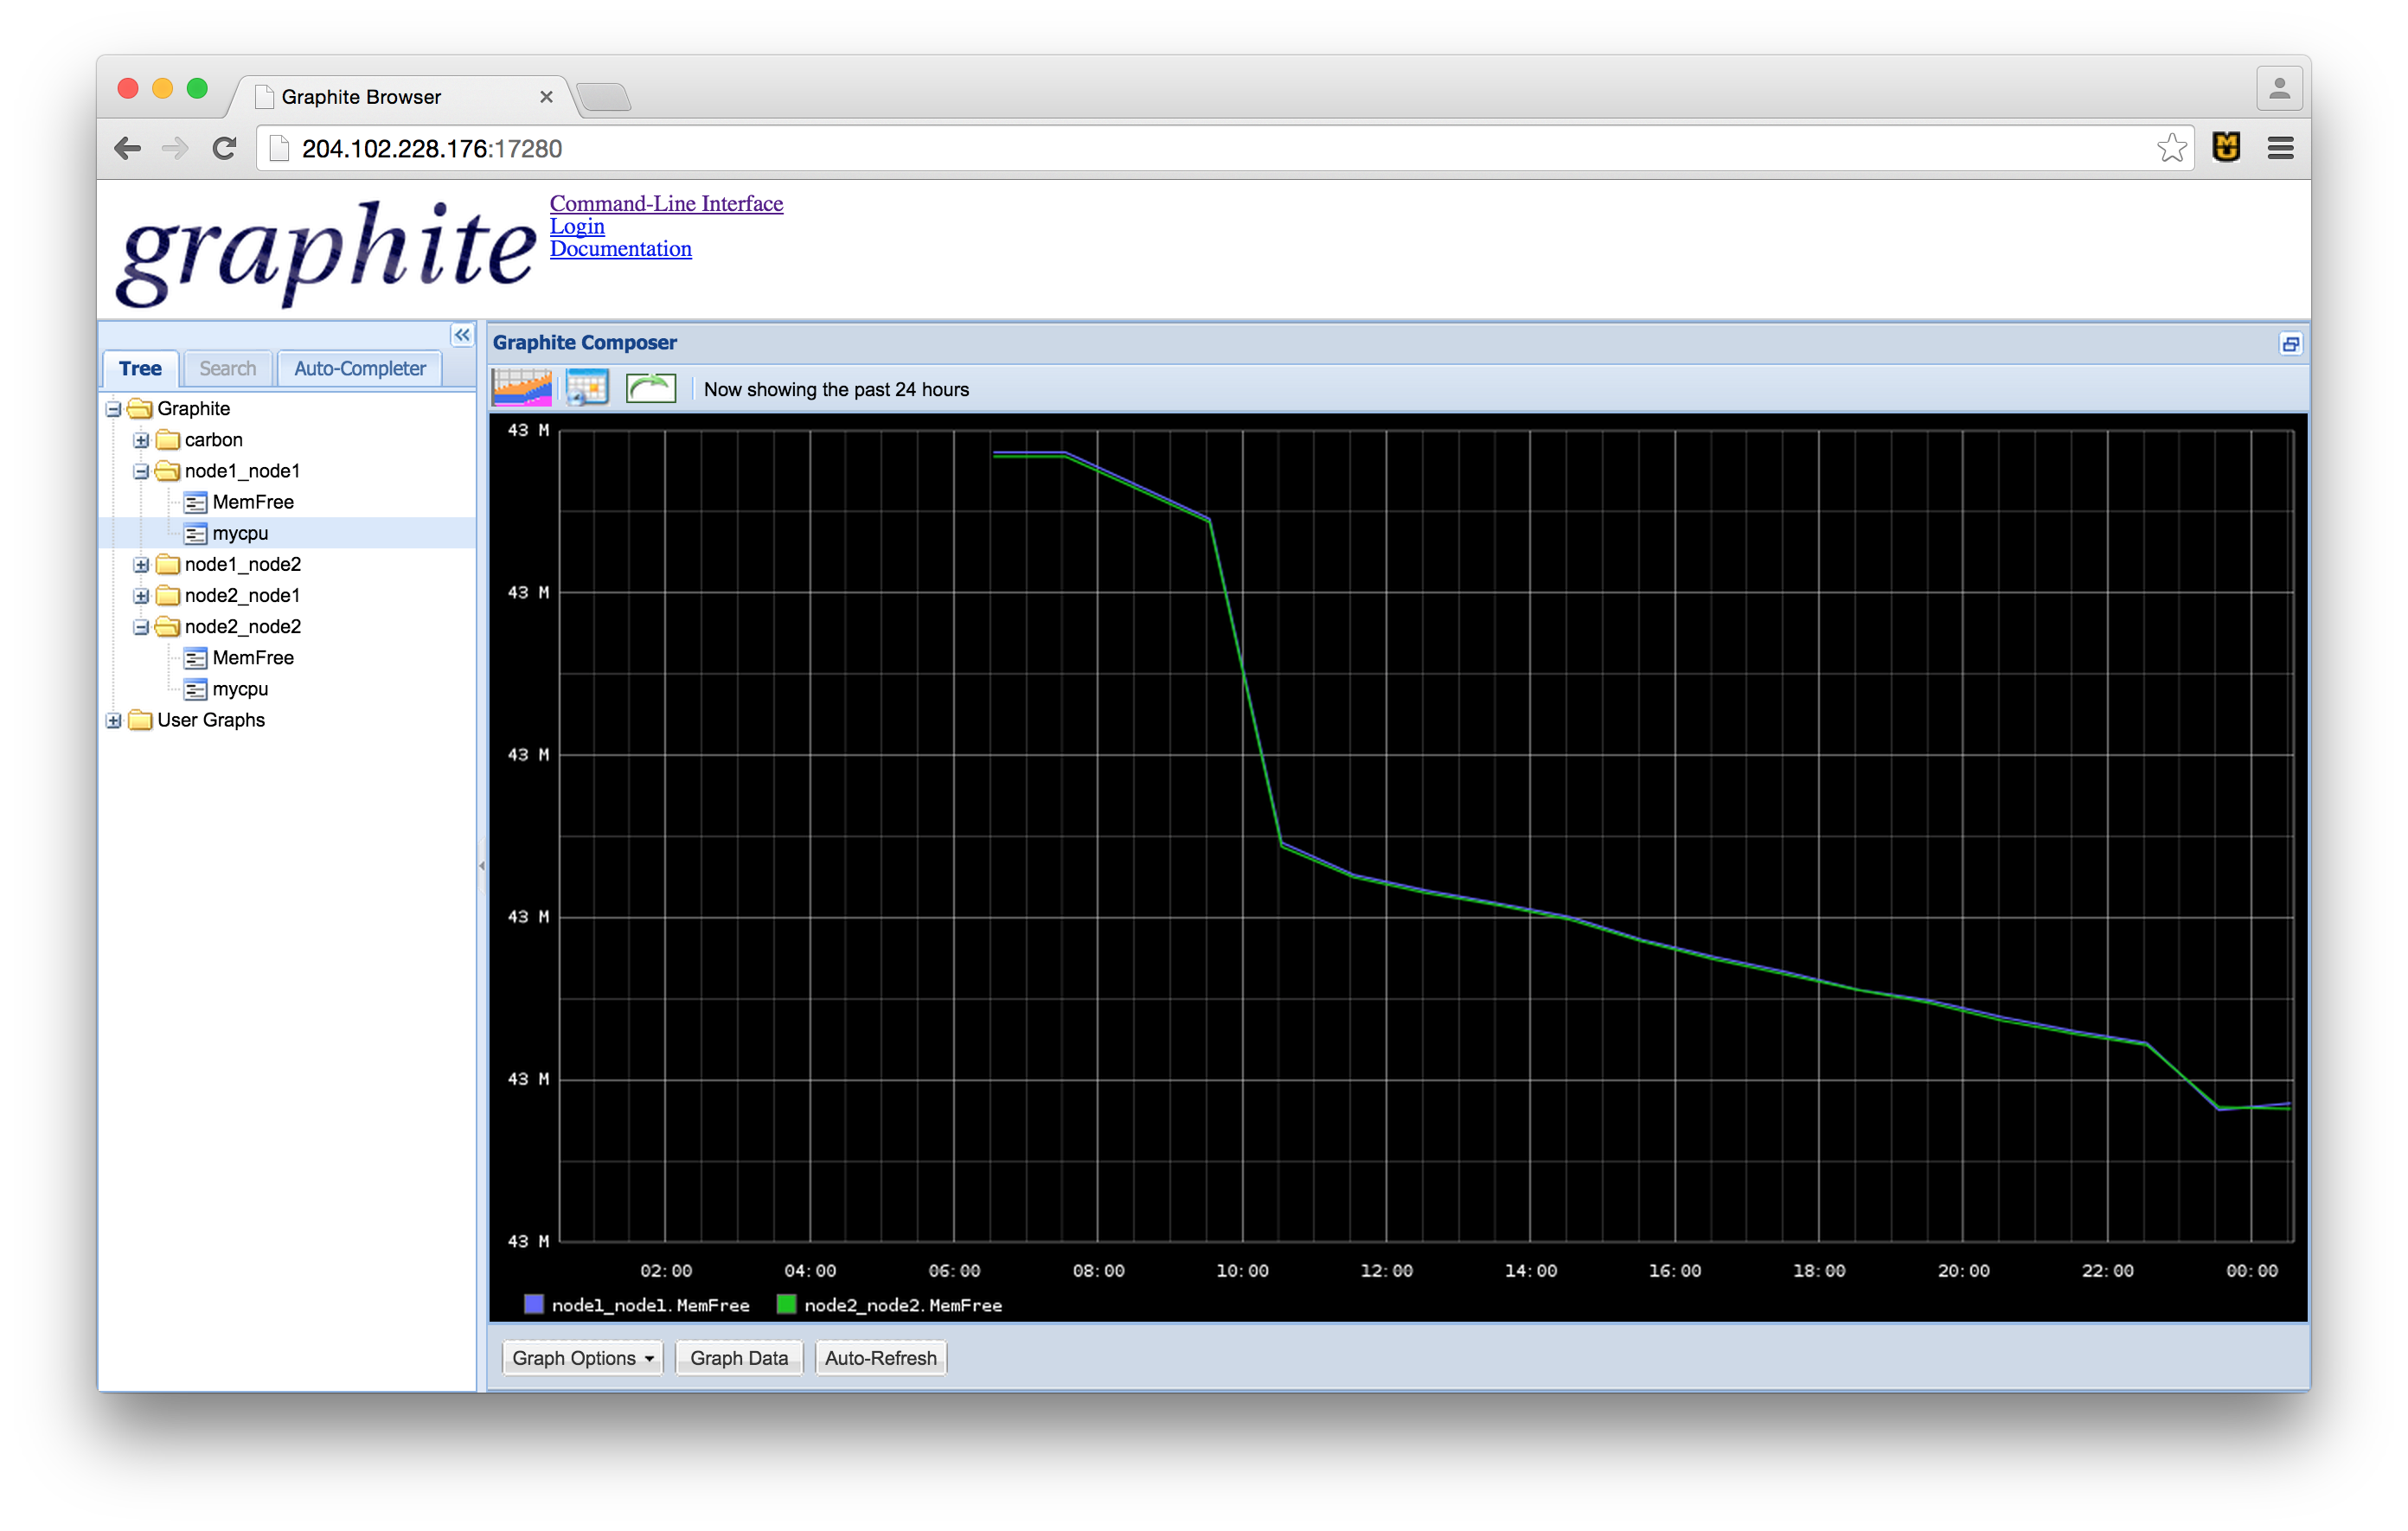
\includegraphics[scale=.32]{memfree.png}
  \caption{MemFree}
\end{figure}
\begin{figure}[H]
  \centering
    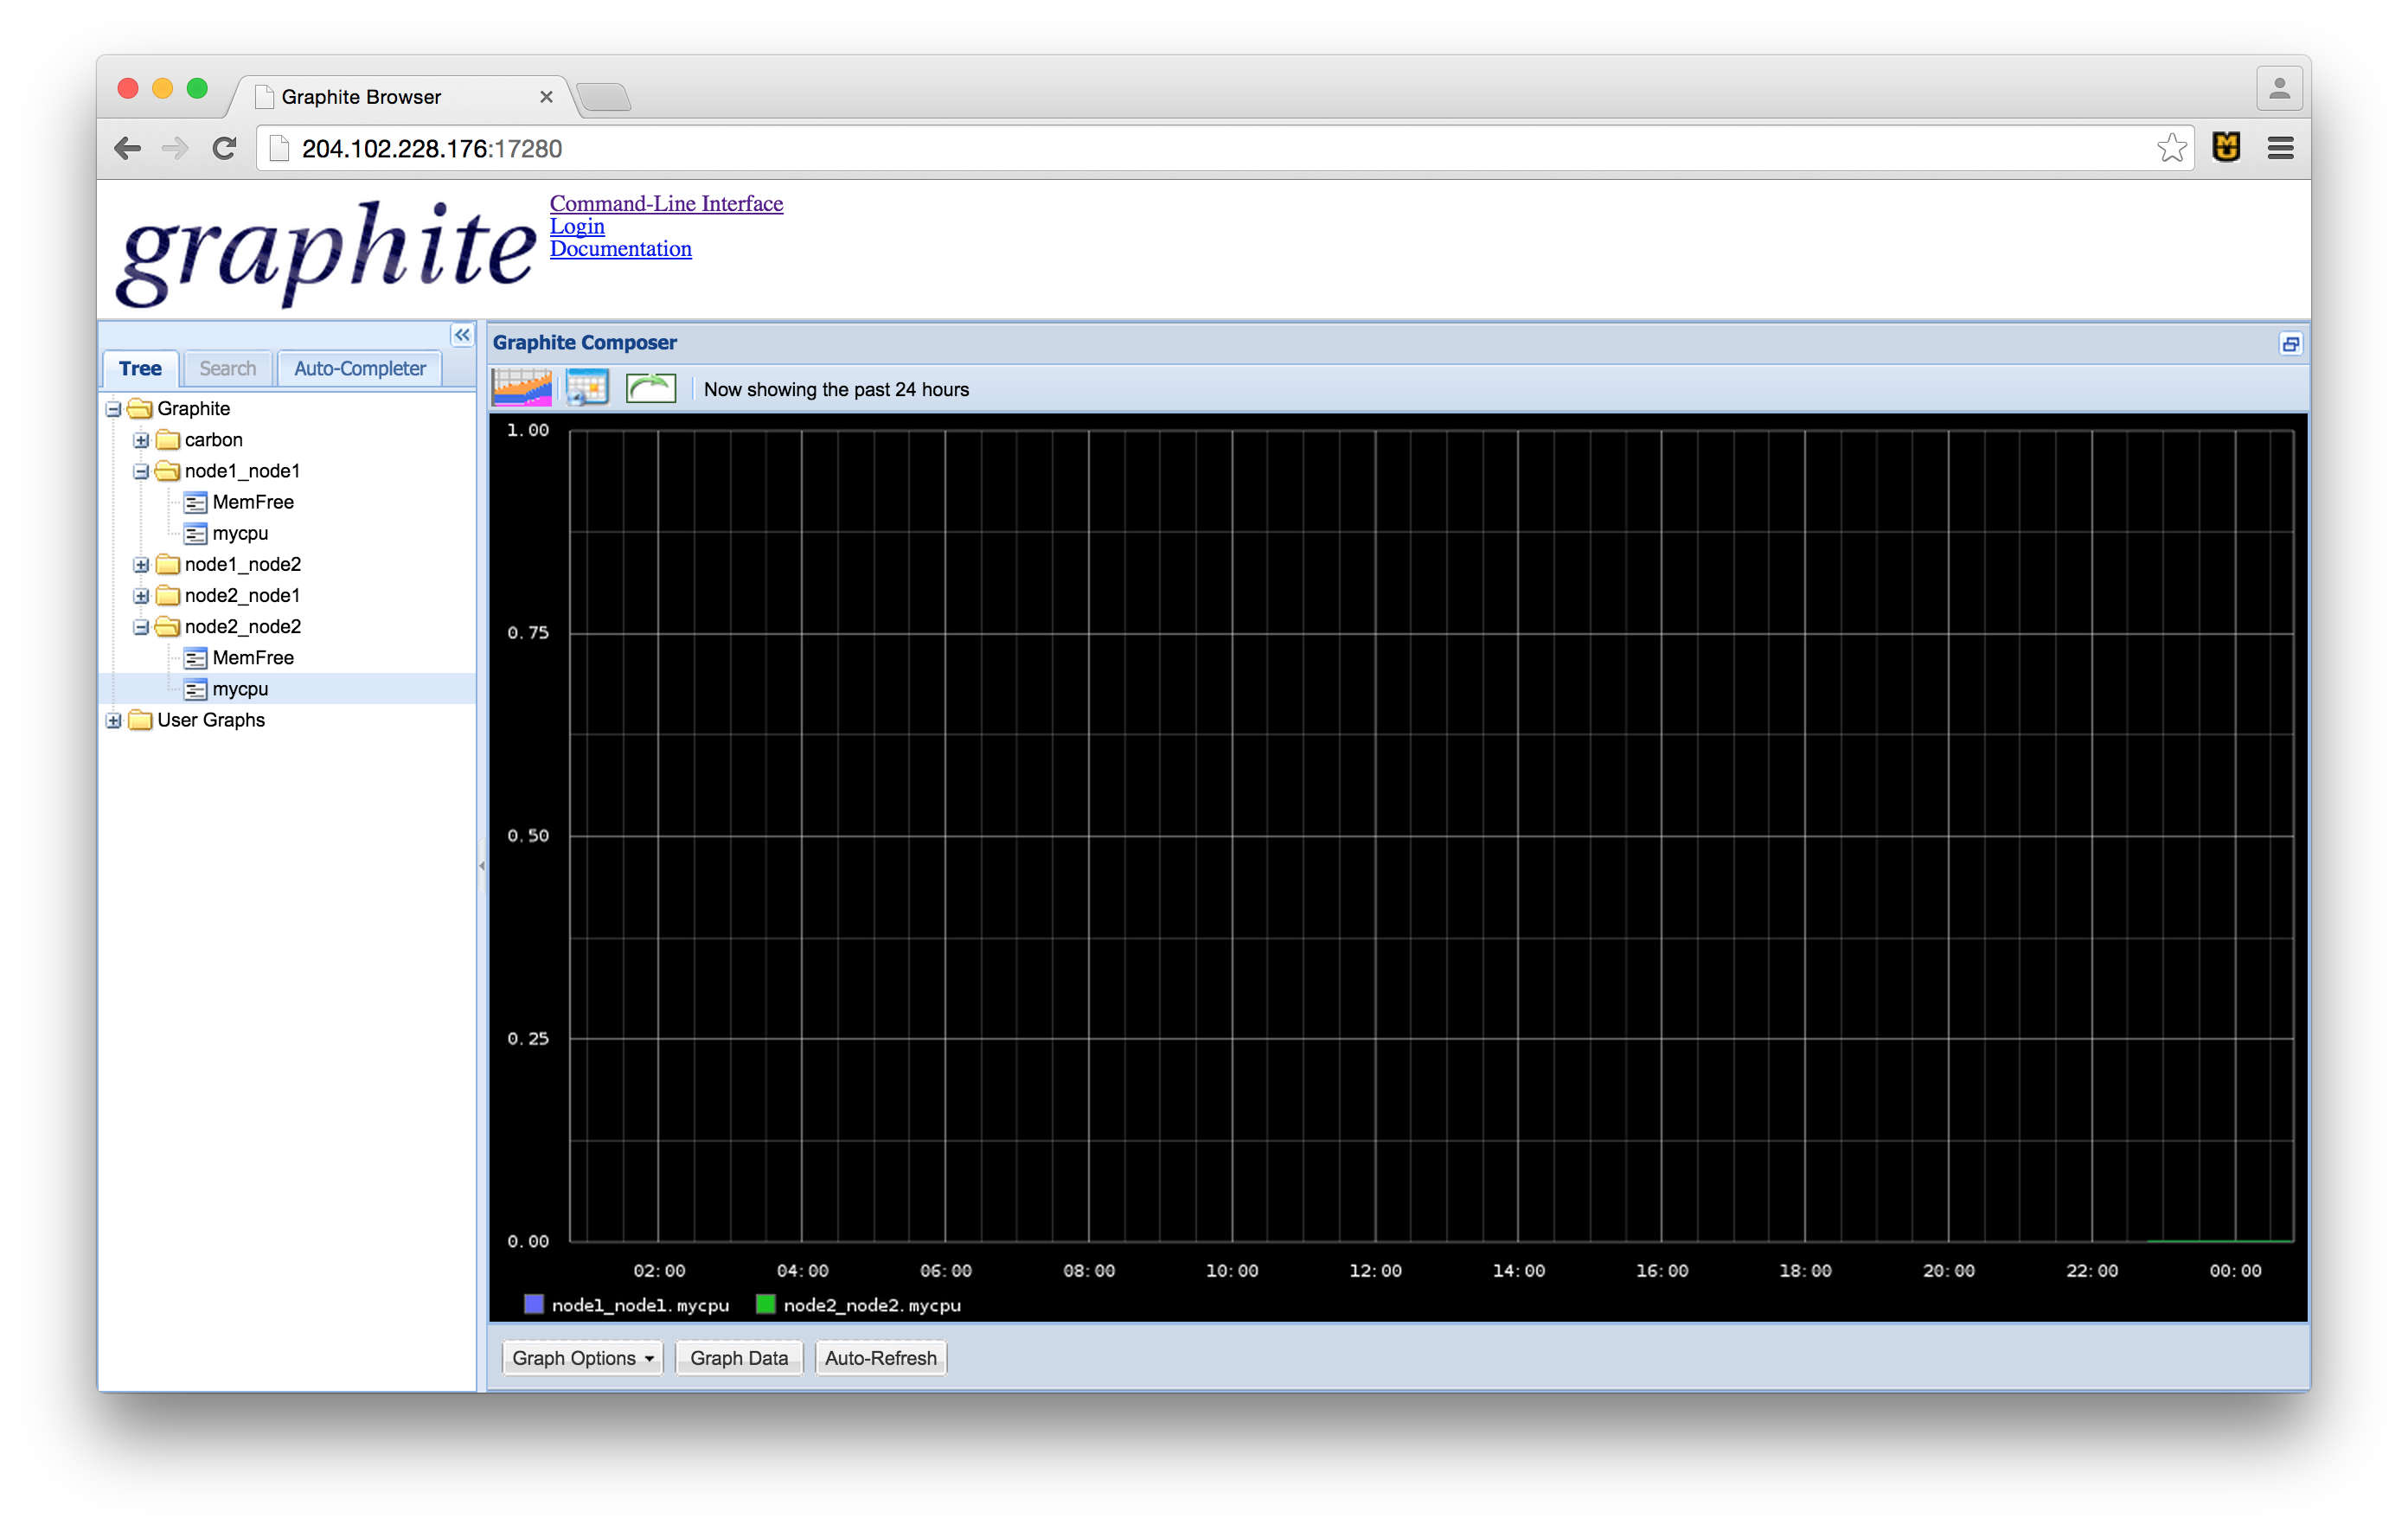
\includegraphics[scale=.32]{mycpu.png}
  \caption{MyCPU on node1 and node2}
\end{figure}

% ---------------------------------------- 2 ----------------------------------------
\paragraph{2. } Explain the role and functions of "Instrumentation and Measurement Tools" such as OnTimeMeasure (http://groups.geni.net/geni/attachment/wiki/OnTimeMeasure/OnTimeMeasure\_Tutorial.pdf?f ormat=raw), and GEMINI Tool Set (http://groups.geni.net/geni/attachment/wiki/GEMINI/gemini-gec13.pptx?format=raw) in GENI infrastructure.

% ---------------------------------------- 3 ----------------------------------------
\paragraph{3. } Briefly explain in your own words the architecture of the 'OnTimeControl' framework (see Reference [3]).

% ---------------------------------------- 4 ----------------------------------------
\paragraph{4. } Describe the workflow that was involved when you added the custom metric feature to your OnTimeMeasure framework instance in the last step of your GENI experiment.

\end{document}